\begin{frame}{a TCP connection}
\begin{tikzpicture}
\tikzset{
    overlay box/.style={fill=white,fill opacity=0.9},
}
\node[overlay,anchor=north west,inner sep=0mm] (base) at (0, 0) {%
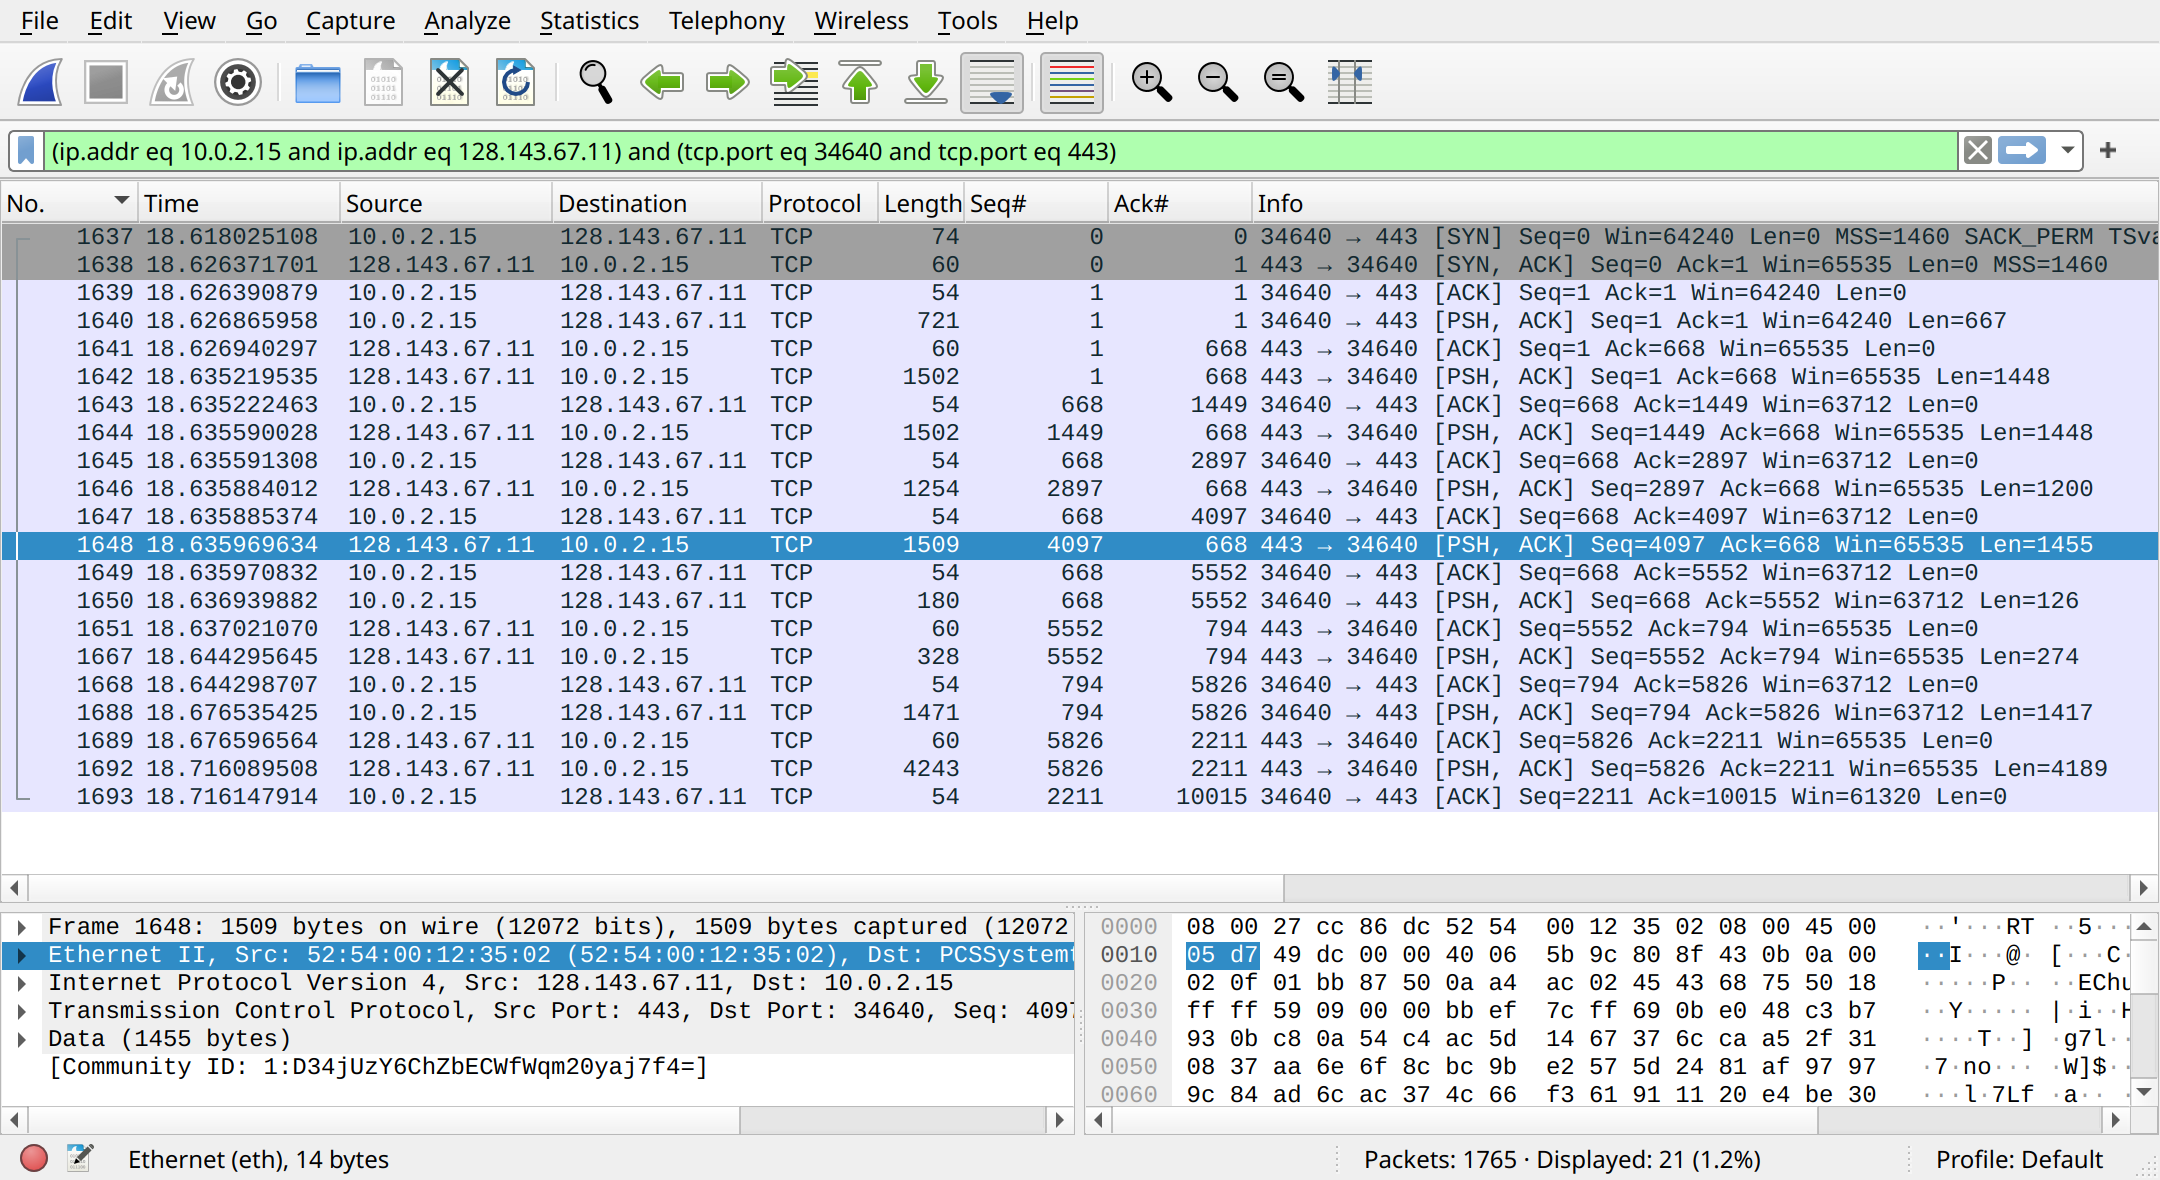
\includegraphics[width=\textwidth]{../reliable/wireshark-tcp-ex1-over}%
};
\path (0, 0) rectangle (14.5, -7); % for bounding box
\draw[overlay,help lines] (0, 0) grid (14, -8);
\begin{visibleenv}<2>

\end{visibleenv}
\end{tikzpicture}
\end{frame}
